\chapter{Implementácia}

Nasledujúca kapitola sa bude zaoberať popisom implementácie dvoch programov pre snímanie prechodov ľudí cez virtuálnu bránu. Prvý program je založený na základe snímania hĺbkovej mapy pomocou hĺbkomeru a druhý na použití bežnej RGB web kamery.

\section{Programovací jazyk a využité knižnice}
Pri implementácii oboch programov bol zvolený programovací jazyk \textit{Python 3}\footnote{Skriptovací jazyk \url{https://www.python.org}} v spojení s knižnicou \textit{OpenCV}\footnote{Computer vision knižnica  \url{http://opencv.org}}. Je to knižnica vytvorená pre počítačové videnie a strojové učenie, distribuovaná pod BSD licenciou. Kladie veľký dôraz na aplikácie bežiace v reálnom čase. 

\section{Výpočetná základňa aplikácie}
Z dôvodu minimalizácie ceny zariadenia bola zvolená ako primárna platforma \textbf{RasperryPi vo verzií 3}. 

Ide o malý počítač, za ktorým stojí britská nadácia s rovnomenným názvom, Raspbery PI. Postavený je na  integrovanom Broadcom SoC procesore BCM2837, ktorý má štyri 1.2 GHz 64-bitové ARM Cortex-A53 jadrá. Ďalšími parametrami sú 1 GB RAM, 100 Mbps Ethernet port, štyri USB 2.0 porty, HDMI výstup. Cena sa pohybuje okolo 35 EUR.

Avšak z dôvodu absencie USB 3.0 boli pri realizácií využité aj iné počítačové platformy.

\section{Implementácia aplikácie s využitím hĺbkového snímania}
Vstupom algoritmu je séria šedotónových hĺbkových obrazov, kde hodnota každého pixlu vyjadruje vzdialenosť od objektu v scéne. Takýto obraz sa nazýva \textit{surová hĺbková mapa} (obrázok \ref{sec:deep_image}). Program tento obraz ďalej spracováva v nasledujúcich dôležitých etapách: 

\begin{itemize}
\item Prahovanie
\item Nájdenie kontúr
\item Priradenie kontúr objektom
\item Sledovanie objektu 
\end{itemize}


\begin{figure}[H]
\begin{center}
	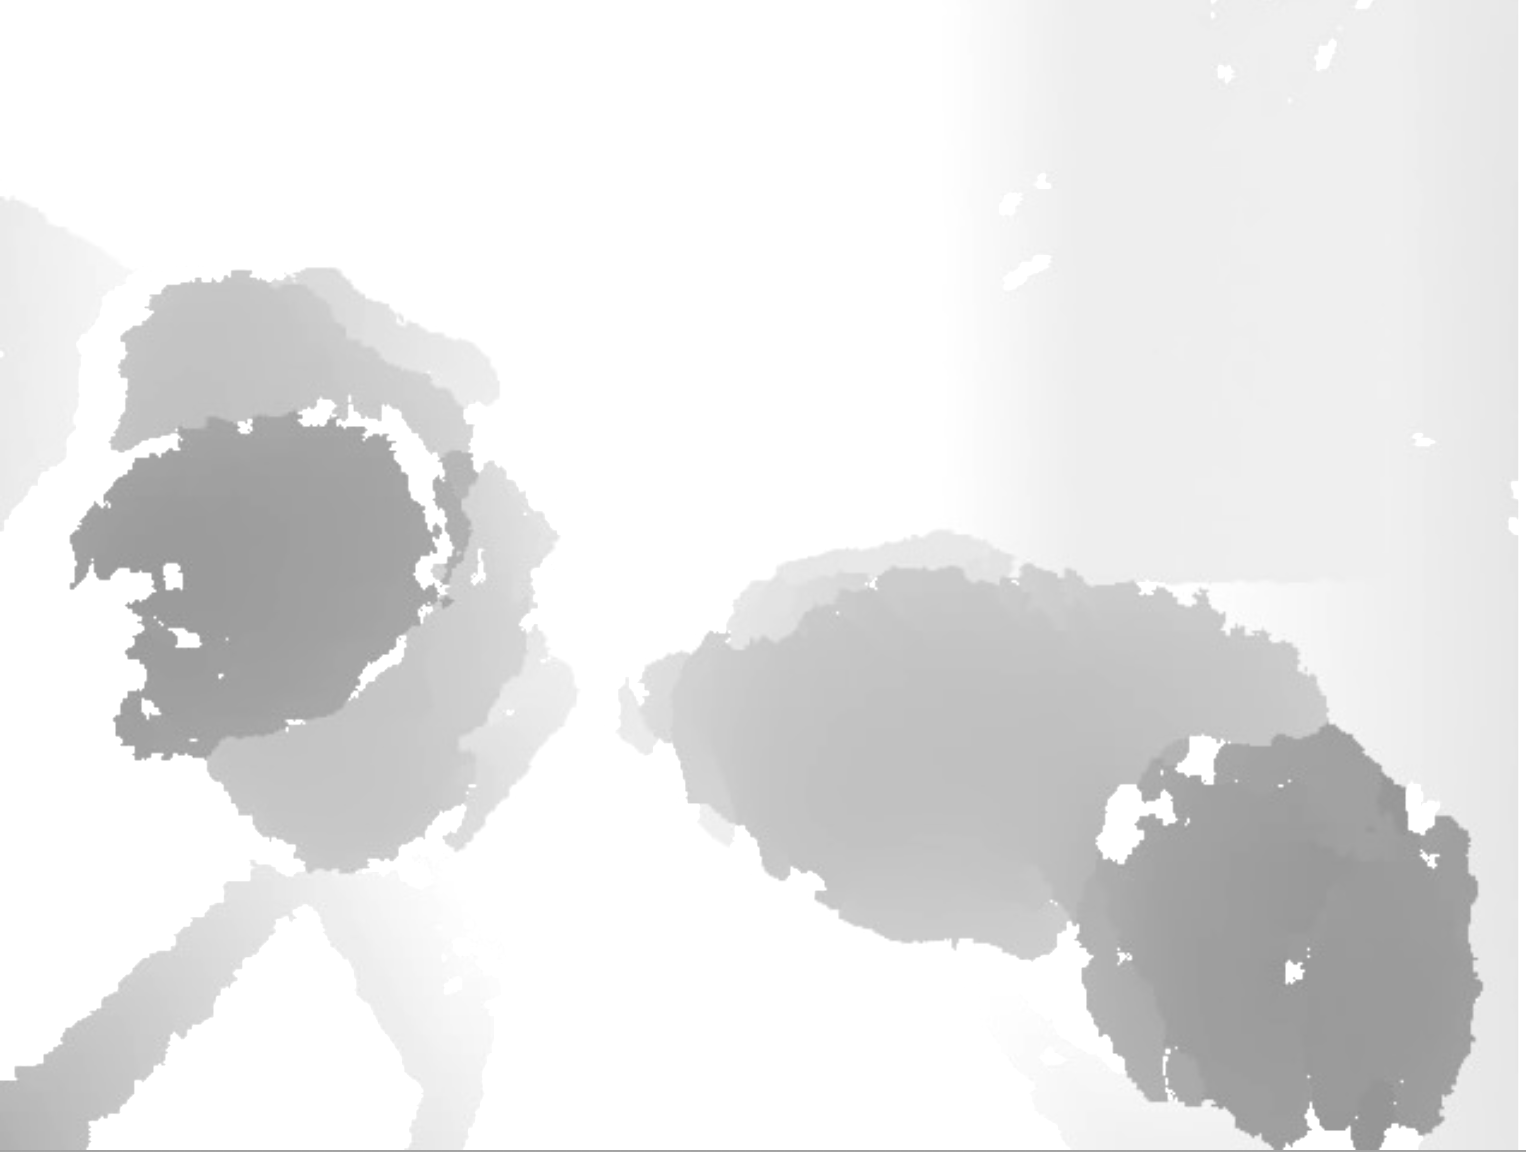
\includegraphics[scale=0.30]{images/deepImage}
	\caption{Surová hĺbková mapa.}
	\label{sec:deep_image}
	\end{center}
\end{figure}



\subsection{Prahovanie}
\label{sec:imp_treashold}
Prahovanie je prvý krok algoritmu. Výstupom je binárna reprezentácia obrazu, kde záujmové body sú reprezentované log 1 a body, ktoré sú nezaujímavé (predmety nemmené, súčasť scény) reprezentované log 0 (obrázok \ref{sec:binary_mask}). Na vstupe fázy algoritmu je surová hĺbková mapa, kde každý pixel predstavuje vzdialenosť od objektu scény. Vďaka tomu môžeme využiť jednoduchý algoritmus globálneho prahovania (kapitola \ref{sec:treasholding}), kde prahová hodnota reprezentuje minimálnu výšku pixlov, ktoré je možno označiť za záujmové. Táto hodnota je súčastou konfiguračných hodnôt, ktoré je nutné nastaviť pri inštalácií aplikácie na prevádzkové miesto. Na prahovanie program využíva funkciu z knižnice opencv \textit{cv2.threshold(grayFrame, MIN\_HEIGHT, 255, cv2.THRESH\_BINARY\_INV)} kde \textit{grayFrame} je snímka hĺbkovej mapy \textit{MIN\_HEIGHT} je hodnota minimálnej výšky. Ďalší argument je hodnota logickej 1 vo výslednej binárnej maske a posledný argument je podmienka určenia $log 1$ alebo $log 0$.

Samostatným problémom metódy globálneho prahovania je, že v scéne môžu existovať predmety, ktoré sú umiestnené v podobnej výške a metóda nie je dostatočná na ich odfiltrovanie. Za týmto účelom sa pri štarte programu vytvorí referenčný snímok scény a pred samotným použitím prahovania sa vyráta absolútny rozdiel medzi referenčným a aktuálnym snímkom. Opísaná funkčnosť je zaistená volaním funkcie \textit{cv2.absdiff(gray\_frame, bg\_reference)}.


\subsection{Nájdenie kontúr}
Cieľom tejto časti spracovania je nájsť kontúry, ktoré korelujú s osobami prechádzajúcimi cez virtuálnu bránu. Vstupom funkcie je binárny obraz vytvorený v \ref{sec:imp_treashold} a výstupom sú kontúry a ich  ťažiská. Činnosť tejto fázy možno rozdeliť do nasledujúcich bodov:  
\begin{itemize}
\item Nájdenie kontúr na základe metódy sledovania hranice (sekcia \ref{sec:follow_border})
\item Spájanie roztrieštených kontúr
\item Filtrácia nevyhovujúcich kontúr
\item Výpočet najvyššieho bodu 
\end{itemize}
\vspace{5mm}

\subsubsection{Hľadanie a spájanie kontúr}
Na základe binárneho obrazu, aplikujeme metódu sledovania hraníc \textit{cv2.findContours}, ktorá je súčastou openCV knižnice. Jej výsledkom je zoznam všetkých uzavretých blobov (kontúr), ktoré sa v binárnom obraze nachádzajú. V dôsledku šumu a nedokonalého snímania hĺbkovej kamery však dochádza k vzniku falošných kontúr a rozpadu objektu na veľké množstvo malých kontúr, ktoré ho reprezentujú. Preto je nutné nájsť spôsob ako tieto chyby napraviť. \vspace{5mm}

\textbf{Spájanie kontúr} - rekurzívny algoritmus, ktorý má za úlohu prehľadať dáta a spojiť kontúry, ktoré potencionálne reprezentujú jeden objekt. 

\begin{figure}[H]
  \centering
  \begin{minipage}[b]{0.45\textwidth}
    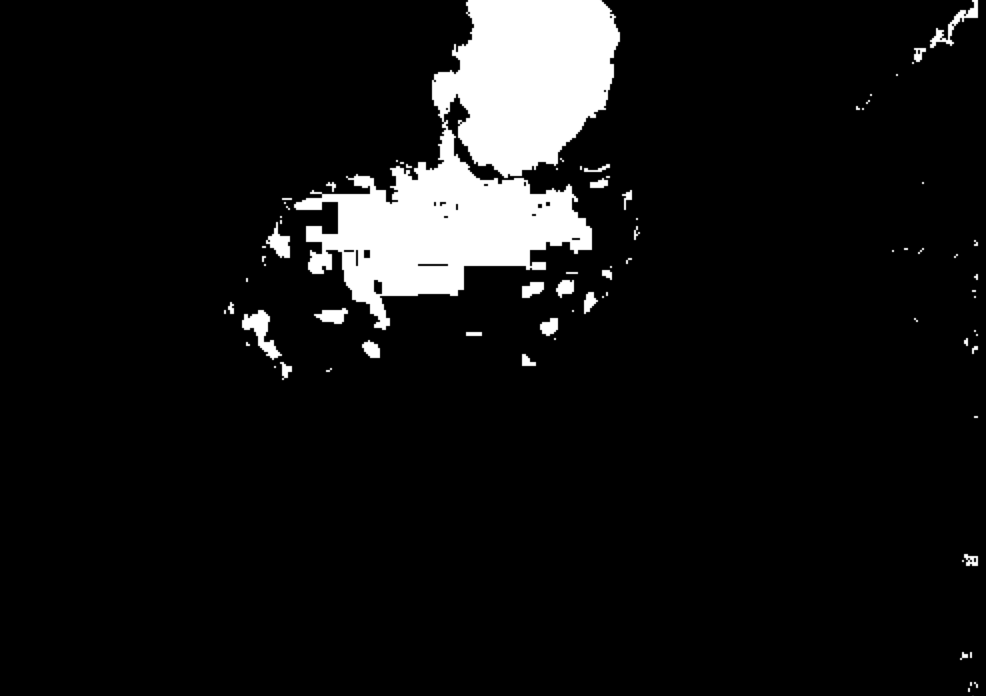
\includegraphics[width=\textwidth]{images/destroyMask}
    \caption{Roztrieštená binárna maska.}
    \label{sec:binary_mask}
  \end{minipage}
  \hfill
  \begin{minipage}[b]{0.4\textwidth}
    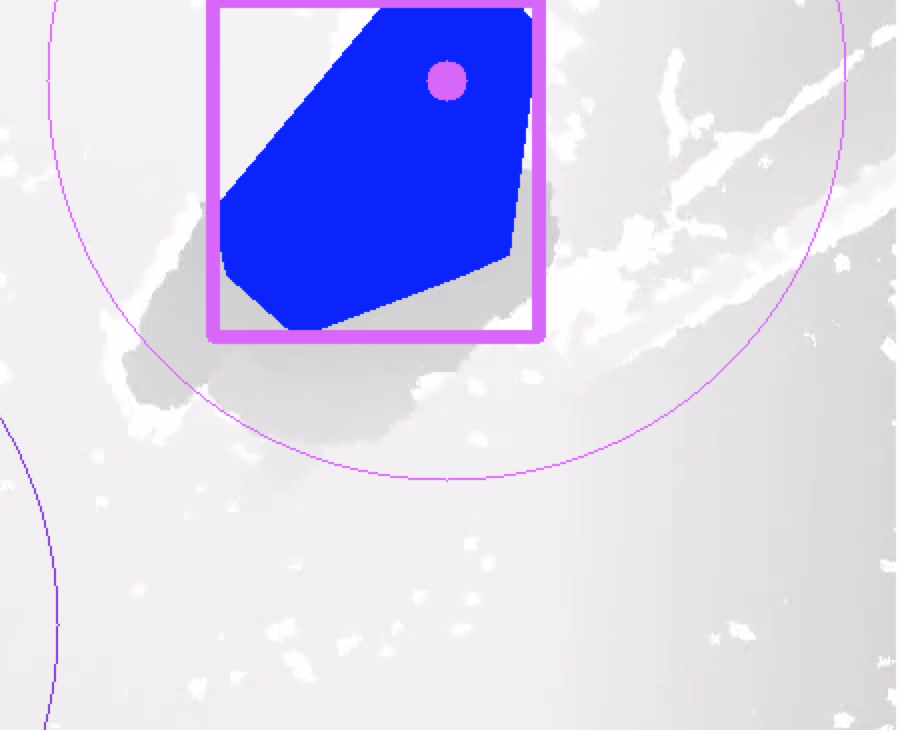
\includegraphics[width=\textwidth]{images/connectMask}
    \caption{Spojená kontúra.}
  \end{minipage}
\end{figure}


Popis algoritmu, pričom všetky kontúry nájdené prostredníctvom funkcie metódy sledovania hraníc, sú uložené v zozname \textit{allCont}:
\begin{enumerate}
  \item Zo zoznamu \textit{allCont} odstránime všetky kontúry, ktoré majú nulový obsah.
  \item Vytvoríme nový zoznam \textit{newContura}, vyberieme prvú kontúru z \textit{allCont}, vložíme do zoznamu \textit{newContura} a označíme ju ako \textit{root}.
  \item V zoznamu \textit{allCont} nájdeme všetky kontúry vyhovujúce podmienke minimálnej absolútnej vzdialenosti ťažísk kontúr oproti kontúre označenej ako \textit{root}.
  \item Nájdené položky vložíme do zoznamu \textit{newContura}, ostatné označíme ako nový zoznam
  \textit{allCont}.
  \item Pre každú najdenú kontúru označíme ako \textit{root} a  pokračuj bodom 3.
  \item Všetky kontúry v zozname \textit{newContura} spojíme do jednej kontúry.
  \item Pre každú konturu v zozname \textit{allCont} pokračujeme bodom 2.
  
\end{enumerate}
Inými slovami, algoritmus prechádza všetky kontúry a na základe vzdialenosti ťažiskových bodov ich spája do jedného celku.


Spájanie zoznamu kontúr je realizované prostredníctvom volania funkcie \textit{cv2.convexHull}, ktorá pre množinou bodov, ktoré sú obrysové body oblasti nájde inú množinu bodov reprezentujúcich jej konvexný obal.

\subsubsection{Filtrácia nevyhovujúcich kontúr}  
Keďže poznáme približnú veľkosť kontúry, ktorej detekcia je cieľom záujmu, všetky ostatné sú nežiaduce a je nutné ich odstrániť. Na základe tejto filtrácie sa program zbaví všetkých náhodných oblastí, ktoré vznikli pôsobením šumu. Túto filtráciu je však možné použiť až po aplikovaní algoritmu pre spájanie kontúr. Je to posledná fáza segmentácie obrazu. 

\subsubsection{Výpočet najvyššieho bodu}
Vďaka tomu, že technológia snímania vytvára hĺbkovú mapu, je možné v rámci každej kontúry definovať lokálne maximum každej oblasti. Pri zvolenej koncepcií snímania, bod patrí do množiny bodov nachádzajúcich sa na vrchnej časti hlavy. Tento bod je významný pri sledovaní pohybu objektu. \vspace{5mm}


Proces nájdenia je definovaný postupom týchto krokov: 
\begin{enumerate}
  \item Vytvoríme prázdnu \textbf{masku} veľkosti snímaného obrazu \textit{np.zeros}.
  \item Do \textbf{masky} vložíme kontúru, ktorej maximálnu oblasť chceme nájsť \textit{cv2.drawContours}.
  \item Nájdeme minimálnu, respektíve maximálnu hodnotu reprezentujúcu najvyšší bod kontúry  \textit{cv2.minMaxLoc(originalFrame, mask=mask)}.
  \item Nájdenú hodnotu použijeme ako prahovú hodnotu a aplikujeme funkciu prahovania s globálnym prahom na originálny obraz. Výsledkom je binárna maska \textit{cv2.threshold}.
  \item Medzi maskou vytvorenou v bode 2 a maskou vytvorenou bode 4 vykonáme logickú operáciu AND, čoho výsledkom je binárna maska maximálnej oblasti skúmanej kontúry \textit{cv2.bitwise\_and(mask, thresh)}.
  \item Následne môžeme znovu vyhľadať všetky uzavrené oblasti, ktoré vznikli na obraze \textit{cv2.findContours}.
  \item Vyberieme kontúru s najväčším obsahom, pre ktorú vyrátame ťažisko a nájdený bod prehlásime za maximálny bod oblasti.
\end{enumerate}

\subsection{Priradenie kontúr objektom}
V prípade, že sme schopní v každom obraze, ktorý patrí do konštantného toku dát zo snímača vykonať spoľahlivú segmentáciu, je možné postúpiť na objektový level abstrakcie. Objekt je určený sériou rôznych kontúr, medzi ktorými existuje vzájomná závislosť.  

Proces vytvárania a zanikania kontúr aplikácie je založený na dvoch hlavných vlastnostiach:
\begin{itemize}
    \item Pozícia oblasti
    \item Hodnota výškového maxima oblasti
\end{itemize}

Pre každý existujúci objekt na scéne sa vypočíta absolútna vzdialenosť ku všetkým nájdeným oblastiam aktuálneho obrazu. Následne sa vzdialenosti usporiadajú od najmenšej po najväčšiu a odstránia všetky, ktoré sú väčšie ako hraničná hodnota stanovená pri konfigurácii. Priradenia, ktoré ostali v zozname sa aplikujú a aktualizuje sa poloha objektov. V prípade, že kontúre nebol priradený žiadny objekt, vytvorí sa nový a kontúra sa priradí ako inicializačná poloha nového objektu. 

\subsection{Sledovanie objektu}
Pri sledovaní osôb v pohybe dochádza k rôznym problémom, ktorým je nutné venovať veľkú pozornosť. Najčastejšie riešeným problémom je jednoznačne určiť, ktorá \textbf{kontúra bude priradená ktorému objektu}. Vzhľadom na to, že priemerný tok dát z kamier je 15 - 20 snímkov za sekundu, zmeny polohy objektov medzi dvoma za sebou idúcimi snímkami môžu byť natoľko veľké, že sledovanie zlyhá. Druhým vážnym problémom je \textbf{spojenie dvoch kontúr do jednej}, čo spôsobuje vytlačenie jedného z objektov, ktorý stratí kontúru, ktorú by mohol sledovať. Táto situácia môže nastať fyzickým kontaktom dvoch osôb (veľmi blízky prechod, zrazenie sa a iné...). Oba problémy majú spoločné riešenie a tým je predikcia nasledujúcej polohy na základe smeru a rýchlosti, ktorú objekt nadobudol do momentu incidentu.
V rámci implementácie som otestoval dva algoritmy.
\begin{itemize}
    \item Kalmanov filter
    \item Výpočet na základe histórie a rýchlosti
\end{itemize}


\begin{figure}[H]
  \centering
  \begin{minipage}[b]{0.4\textwidth}
    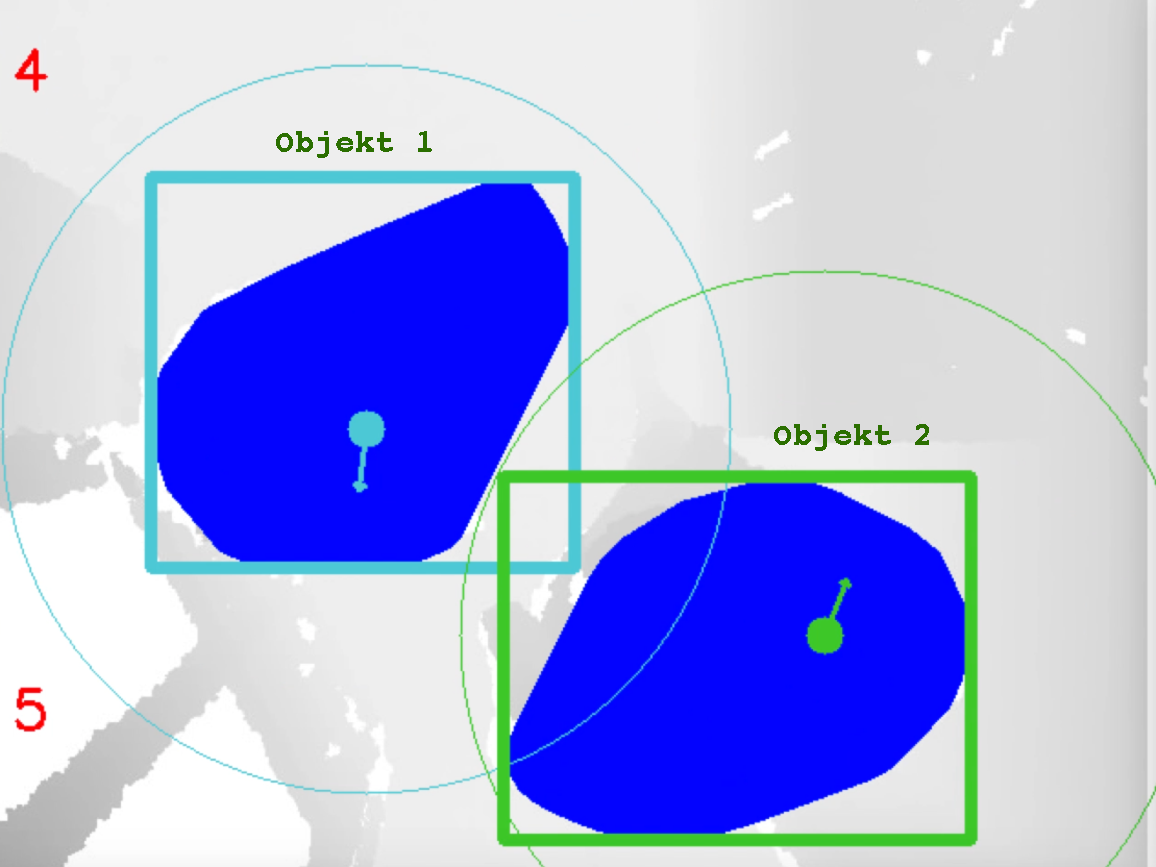
\includegraphics[width=\textwidth]{images/beforeCollision}
    \caption{Moment pred kolíziou dvoch kontúr.}
  \end{minipage}
  \hfill
  \begin{minipage}[b]{0.55\textwidth}
    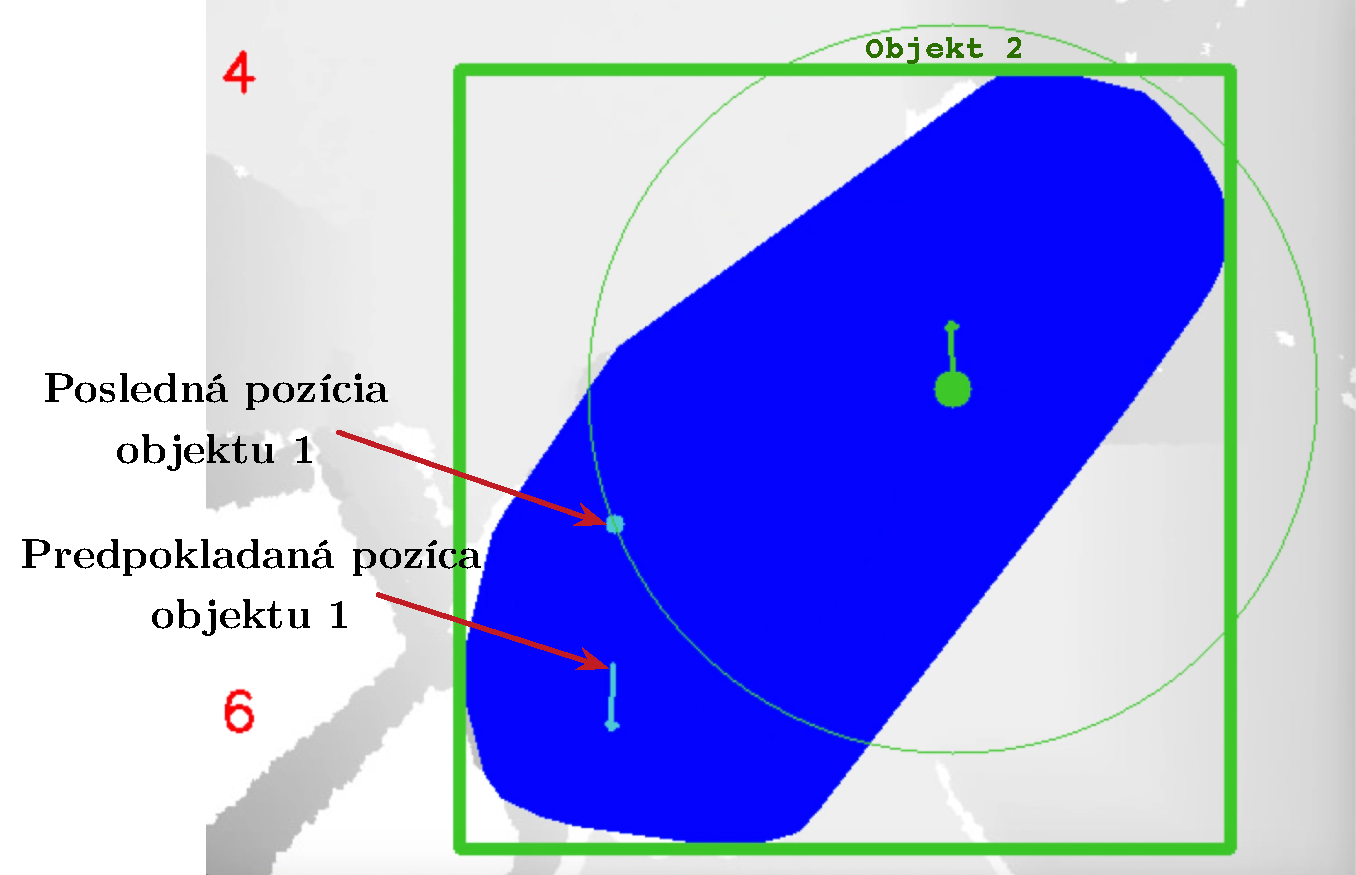
\includegraphics[width=\textwidth]{images/predicate}
    \caption{Využitie predpovedania polohy.}
  \end{minipage}
\end{figure}



\textbf{Kalmanov filter} - Teoretický základ funkčnosti tohto filtra bol opísaný v sekcii \ref{sec:kalman}. Pri implementácii som využil knižnicu \textit{openCV}, ktorá ho obsahuje. Pri testoch som však objavil veľký problém. Kalmanov filter potrebuje pomerne veľkú históriu korekcii na to, aby získal požadovanú presnosť. Priemerný prechod jedného človeka cez virtuálnu bránu, je zachytený na 10 - 20 snímkoch. Podľa testov Kalmanov filter potrebuje na získanie základnej presnosti 5 - 6 korekcii. Tento problém je samozrejme možné riešiť zmenou snímacieho zariadenia alebo umiestnením kamery na vyššie položené miesto, a tým maximalizovať zotrvanie objektov na scéne. 

\textbf{Výpočet na základe histórie a rýchlosti} - Táto metóda je veľmi jednoduchá a opiera sa o vedomosti zo základnej školy. Pre každý objekt vytvoríme históriu, ktorá obsahuje pozíciu a časovú známku. Veľkosť histórie definujeme podľa toho, koľko bodov má ovplyvňovať predikciu nasledujúceho bodu. Proces výpočtu predikcie potom vyzerá tak, že najprv vyrátame moment rýchlosti pre x-ovú aj y-ovú os: 

\begin{figure}[H]
    \centering
    \begin{minipage}[b]{0.45\textwidth}
        \begin{equation}
            v_x = \frac{last_x - first_x} {t}
        \end{equation}
    \end{minipage}
    \hfill
    \begin{minipage}[b]{0.4\textwidth}
        \begin{equation}
            v_y = \frac{last_y - first_y} {t}
        \end{equation}
    \end{minipage}
\end{figure}

kde \textit{last} je najstaršia známa poloha, \textit{first} je najnovšia pozícia a \textit{t} je celkový čas od najstaršieho po najnovší záznam v histórii. Keď máme vypočítané rýchlosti, máme všetko pre určenie predikcie na základe aktuálneho času takto: 

\begin{figure}[H]
    \centering
    \begin{minipage}[b]{0.45\textwidth}
        \begin{equation}
            predicate_x = last_x + v_x * \Delta t
        \end{equation}
    \end{minipage}
    \hfill
    \begin{minipage}[b]{0.4\textwidth}
        \begin{equation}
            predicate_y = last_y + v_y * \Delta t
        \end{equation}
    \end{minipage}
\end{figure}

kde, $\Delta t$ je rozdiel medzi časom hľadanej polohy a časom poslednej známej polohy. Tento výpočet funguje spoľahlivo už pri druhom snímku a pri testoch dosahoval lepšie výsledky ako Kalmanov filter. Z toho dôvodu bol na predikciu polohy využitý práve tento algoritmus. 

\section{Implementácia aplikácie s využitím RGB web kamery}
Implementácia aplikácie s využitím RGB web kamery využíva veľmi podobné stratégie ako aplikácia založená na hĺbkovom snímaní, ktorá bola opísaná vyššie. Dva najvýznamnejšie rozdiely predstavujú:
\begin{itemize}
\item Spôsob vytvárania binárnej masky
\item Určenie významného bodu oblasti - ťažisko oblasti
\end{itemize}

\subsection{Binárna maska}
Princíp snímania webkamery je založený na interakcii CCD čipu  so svetlom prichádzajúcim od pozorovaného objektu. Odrazom svetla od povrchu sa môže odraziť v plnom spektre pod rovnakým uhlom (zrkadlo, lesklé objekty), alebo svetlo prenikne do objektu, kde sa časť vlnovej dĺžky sa pohltí a zvyšok sa odrazí. Senzor teda vníma spektrum odrazeného svetla ako určitú farbu.

Ak by sme aj v tomto prípade chceli využiť \textbf{metódu prahovania}, museli by sme zabezpečiť, aby priestor snímaný kamerou bol vždy farebne iný od objektov prechádzajúcich skrz. Tak by bolo možné odfiltrovať všetky pixle s vlnovou dĺžkou odrazeného svetla (farbou) zodpovedajúcou pozadiu. Ďalej by bolo nutné zabezpečiť homogénne osvetlenie scény, aby bol zabezpečený dostatok svetla. Vzhľadom na všetky tieto problémy je metóda nepoužiteľná pre daný účel.

Výhodnejšou stratégiou predstavuje použitie \textbf{metódy odčítavania pozadia} (\textit{Background Subtractor}). Je to analytická metóda, pre postupné učenie sa pozadia a jeho odčítavanie od obrazu v popredí. Výsledkom je binárna maska obrazu, kde pixel, ktorý sa zmenil má logickú hodnotu 1 a pixel, ktorý je pozadím 0. 

\subsubsection{Požiadavky na výkon}
Algoritmy pre odčítavanie pozadia sú veľmi náročné na výpočtový výkon a to priamoúmerné na rozlíšeniu spracovávaného obrazu. V rámci implementácie boli testované MOG\footnote{Odkaz na publikáciu: \url{http://link.springer.com/chapter/10.1007\%2F978-1-4615-0913-4_11}}, MOG2\footnote{Odkaz na publikáciu: \url{http://ieeexplore.ieee.org/document/1333992/}}, KNN.

Najlepší pomer kvality binárnej masky a výkonu potrebného na jej získanie má \textit{KNN (K-nearest)}. Jeho implementáciu obsahuje knižnica  \textit{cv2.createBackgroundSubtractorKNN()}. Je veľmi efektívny, ak sa v popredí obrazu mení len jeho malá časť. 

\subsubsection{Paralelné spracovávanie}
Pri implementácii ďalších testoch sa však ukázalo, že pri spustení aplikácie na Rasperry PI rýchlosť spracovávania jednotlivých obrazov bola nedostatočná (8-10 FPS). Pre zvýšenie priepustnosti spracovávania bolo nutné zlepšiť vyťaženie viacerých jadier procesora súčasne (asynchrónny prístup). 

Implementácia asynchrónneho spracovania funguje na princípe generácie množstva vlákien, ktoré sú spolu synchronizované na základe zámkov. V prvom kroku algoritmu sa inicializuje \textit{videostream} a \textit{background substractor}. Následne sa vygeneruje N vlákien (\textit{workers}). Každé vlákno obsahuje jeden zámok na čítanie ďalšieho snímku obrazu a druhý zámok pre zápis do zoznamu spracovaných snímkov. Tie sa pri vytváraní uzamknú. Každé vlákno v nekonečnom cykle vykonáva:
\begin{enumerate}
\item Uzamknutie zámku pre čítanie ďalšieho snímku
\item Čítanie ďalšieho snímku 
\item Otvorenie zámku pre čítanie nasledujúceho vlákna \textit{(i + 1)}
\item Zahájenie výpočtu Bacground substractoru
\item Uzamknutie zámku pre zápis výsledku do zoznamu výsledkov
\item Vloženie výsledku operácie do zoznamu výsledkov 
\item Otvorenie zámku pre vloženie výsledku ďalšieho vlákna \textit{(i + 1)} 
\end{enumerate}

Algoritmus bol testovaný na \textit{Raspberry PI 3}. Nasledujúce grafy prezentujú závislosť rýchlosti spracovávania snímkov na veľkosti snímaného obrazu a počte vlákien algoritmu:

\begin{figure}[H]
  \centering
  \begin{minipage}[b]{0.49\textwidth}
    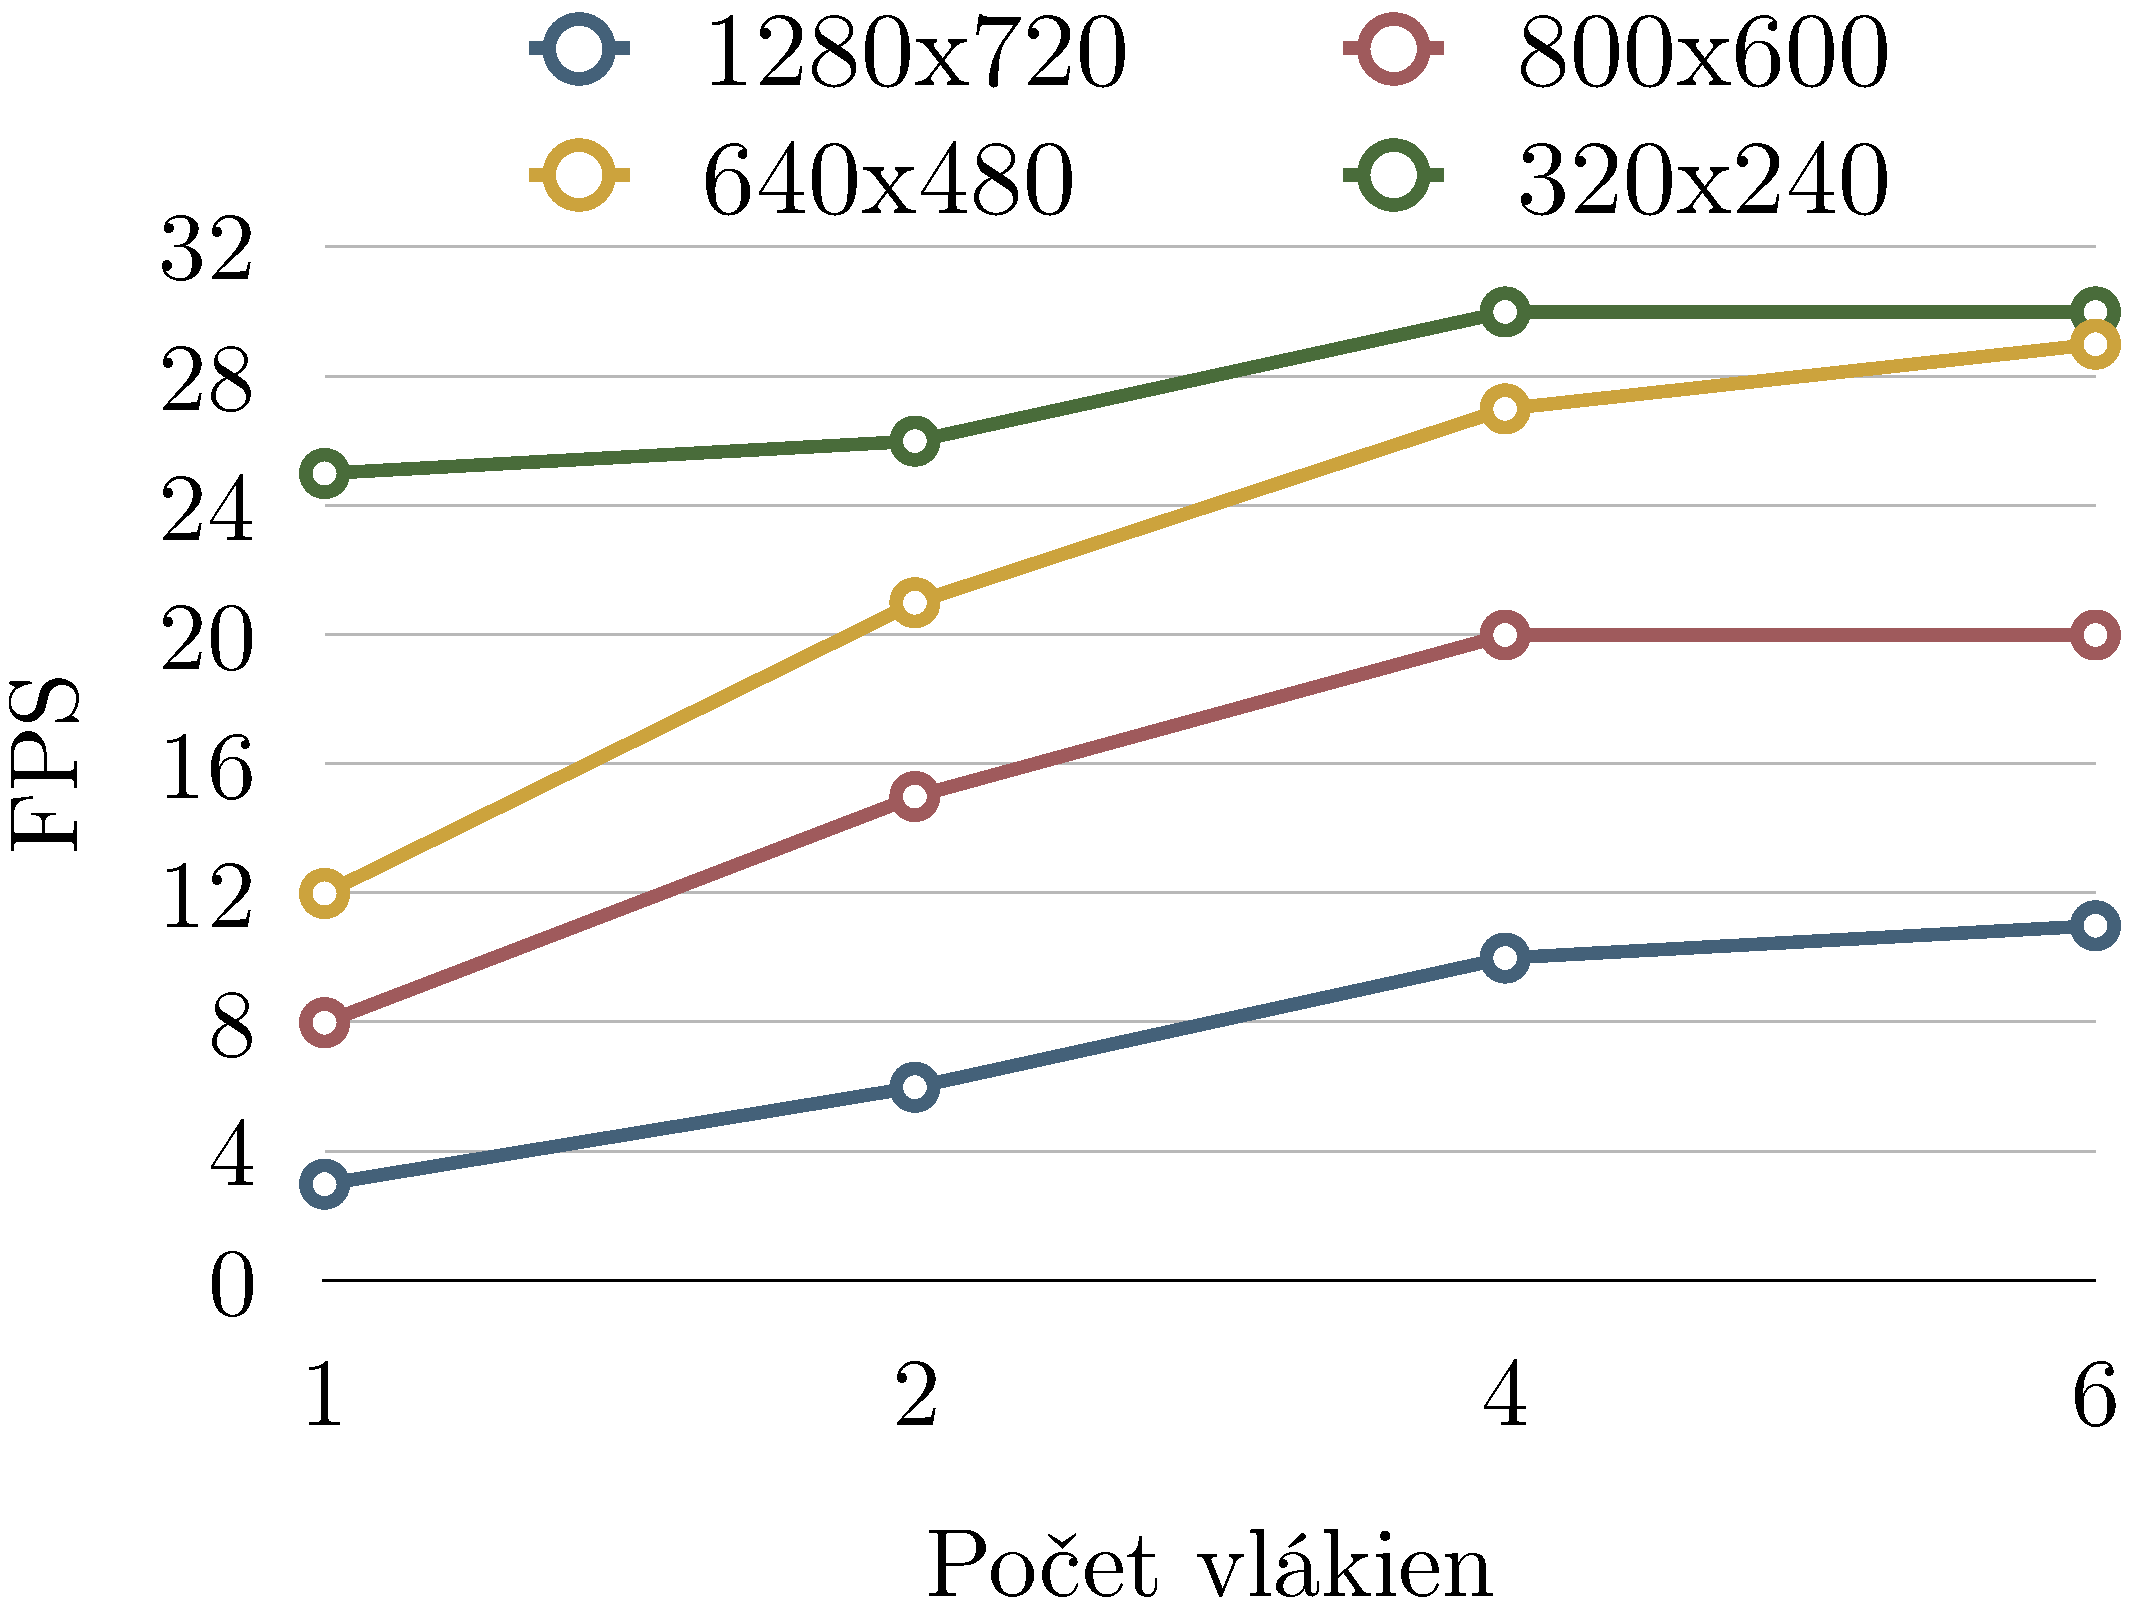
\includegraphics[width=\textwidth]{images/substractorCalm}
    \caption{Nemenná scéna.}
  \end{minipage}
  \hfill
  \begin{minipage}[b]{0.49\textwidth}
    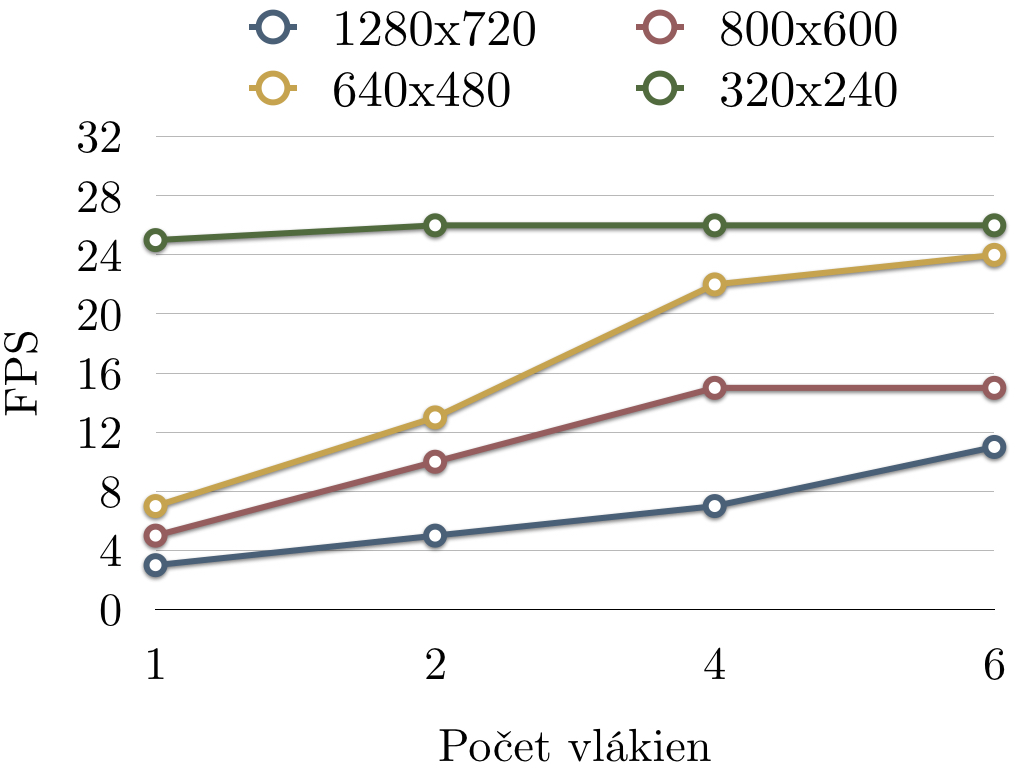
\includegraphics[width=\textwidth]{images/substractorNormal}
    \caption{Priemerne veľký pohyb na scéne.}
  \end{minipage}
\end{figure}

Z testov vyplýva, že algoritmus najlepšie pracuje pri snímacom rozlíšení \textbf{640*480 pixlov} s využitím \textbf{štyroch asynchrónnych vlákien}. Pri týchto atribútoch dosiahnutá hodnota snímkov za sekundu (FPS) aj veľkosť rozlíšenia dostatočná pre ďalšie spracovanie. 



